% \documentclass[11pt]{aghdpl}
\documentclass[en,11pt]{aghdpl}  % praca w języku angielskim

% Lista wszystkich języków stanowiących języki pozycji bibliograficznych użytych w pracy.
% (Zgodnie z zasadami tworzenia bibliografii każda pozycja powinna zostać utworzona zgodnie z zasadami języka, w którym dana publikacja została napisana.)
\usepackage[polish,english]{babel}

% Użyj polskiego łamania wyrazów (zamiast domyślnego angielskiego).
% \usepackage{polski}

\usepackage[utf8]{inputenc}

% dodatkowe pakiety

\usepackage{mathtools}
\usepackage{amsfonts}
\usepackage{amsmath}
\usepackage{amsthm}
\usepackage{hyperref}

% --- < bibliografia > ---

\usepackage[
style=numeric,
sorting=none,
% Zastosuj styl wpisu bibliograficznego właściwy językowi publikacji.
language=autobib,
autolang=other,
% Zapisuj datę dostępu do strony WWW w formacie RRRR-MM-DD.
urldate=iso,
seconds=true,
% Nie dodawaj numerów stron, na których występuje cytowanie.
backref=false,
% Podawaj ISBN.
isbn=true,
% Nie podawaj URL-i, o ile nie jest to konieczne.
url=false,
% Ustawienia związane z polskimi normami dla bibliografii.
maxbibnames=3,
% Jeżeli używamy BibTeXa:
backend=bibtex
]{biblatex}

\usepackage{fvextra}
\usepackage{csquotes}
% Ponieważ `csquotes` nie posiada polskiego stylu, można skorzystać z mocno zbliżonego stylu chorwackiego.
\DeclareQuoteAlias{croatian}{polish}

\addbibresource{bibliography.bib}

% Nie wyświetlaj wybranych pól.
%\AtEveryBibitem{\clearfield{note}}

% Użyj czcionki kroju Courier.
\usepackage{courier}


% ------------------------

\AtBeginDocument{
	\renewcommand{\tablename}{Table}
	\renewcommand{\figurename}{Picture}
}

% ------------------------
% --- < tabele > ---

\usepackage{array}
\usepackage{tabularx}
\usepackage{multirow}
\usepackage{booktabs}
\usepackage{makecell}
\usepackage[flushleft]{threeparttable}

% defines the X column to use m (\parbox[c]) instead of p (`parbox[t]`)
\newcolumntype{C}[1]{>{\hsize=#1\hsize\centering\arraybackslash}X}

% ------------------------
% --- < glossary > ---

\usepackage[automake, acronyms, toc, nopostdot, nonumberlist, nomain]{glossaries}
\loadglsentries{glossaries}
\makeglossaries
% \glsaddall

% ------------------------
% --- < minted > ---

\usepackage[outputdir=build]{minted}
\definecolor{bg}{rgb}{0.95,0.95,0.95}
\setminted{
  fontfamily=txtt,
  fontsize=\footnotesize,
  samepage=false,
  style=xcode,
  breaklines,
  bgcolor=bg
}
% listings with page breaking
\newenvironment{longlisting}{\captionsetup{type=listing}}{}

% custom lexer for toml
\newminted[tomlcode]{lexers/toml.py:TomlLexer -x}{}
\newmintinline[tomlcodeinline]{lexers/toml.py:TomlLexer -x}{}
\newmintedfile[tomlfile]{lexers/toml.py:TomlLexer -x}{}

% custom lexer for ladr
\newminted[ladrcode]{lexers/ladr.py:LadrLexer -x}{}
\newmintinline[ladrcodeinline]{lexers/ladr.py:LadrLexer -x}{}
\newmintedfile[ladrfile]{lexers/ladr.py:LadrLexer -x}{}

% custom lexer for spass
\newminted[spasscode]{lexers/spass.py:SpassLexer -x}{}
\newmintinline[spasscodeinline]{lexers/Spass.py:SpassLexer -x}{}
\newmintedfile[spassfile]{lexers/spass.py:SpassLexer -x}{}

% custom lexer for tptpt
\newminted[tptpcode]{lexers/tptp.py:TptpLexer -x}{}
\newmintinline[tptpcodeinline]{lexers/tptp.py:TptpLexer -x}{}
\newmintedfile[tptpfile]{lexers/tptp.py:TptpLexer -x}{}
%---------------------------------------------------------------------------

\author{Mateusz Grzeliński}
\shortauthor{M. Grzeliński}

%\titlePL{Przygotowanie bardzo długiej i pasjonującej pracy dyplomowej w~systemie~\LaTeX}
%\titleEN{Preparation of a very long and fascinating bachelor or master thesis in \LaTeX}

\titlePL{System losowego generowania formuł logicznych dla logiki pierwszego rzędu}
\titleEN{System of random generation of logical formulas for first order logic}


\shorttitlePL{Losowy generator formuł logiki pierwszego rzędu}
\shorttitleEN{Random FOL formula generator}

\thesistype{Praca dyplomowa inżynierska}
\thesistype{Bachelor of Science Thesis}

% \supervisor{dr inż. Radosław Klimek }
\supervisor{Radosław Klimek PhD, DSc}

% \degreeprogramme{Informatyka}
\degreeprogramme{Computer Science}

\date{2019}

% \department{Katedra Informatyki Stosowanej}
\department{Department of Applied Computer Science}

% \faculty{Wydział Elektrotechniki, Automatyki,\protect\\[-1mm] Informatyki i Inżynierii Biomedycznej}
\faculty{Faculty of Electrical Engineering, Automatics, Computer Science and Biomedical Engineering}

% \acknowledgements{}


\setlength{\cftsecnumwidth}{10mm}

%---------------------------------------------------------------------------
\setcounter{secnumdepth}{4}
\brokenpenalty=10000\relax

\begin{document}

\titlepages

% Ponowne zdefiniowanie stylu `plain`, aby usunąć numer strony z pierwszej strony spisu treści i poszczególnych rozdziałów.
\fancypagestyle{plain}
{
	% Usuń nagłówek i stopkę
	\fancyhf{}
	% Usuń linie.
	\renewcommand{\headrulewidth}{0pt}
	\renewcommand{\footrulewidth}{0pt}
}

\setcounter{tocdepth}{2}
\tableofcontents
\newpage

\chapter{Introduction}
% \label{cha:Introduction}

The goal of this this thesis is to create random \gls{FOL} generator. User will be able to define:
\begin{itemize}
\item what classes of \gls{FOL} elements want to include
\item how many elements given class should appear in rendered formula (within given threashold)
\end{itemize}

Using this generator the following datasets were created:
\begin{enumerate}
  \item TODO
\end{enumerate}


\section{Formal logical systems}
% https://en.wikipedia.org/wiki/Mathematical_logic#Formal_logical_systems
% https://en.wikipedia.org/wiki/Formal_system#Logical_system
% https://en.wikipedia.org/wiki/Formal_system
% https://cs.lmu.edu/~ray/notes/formalsystems/

A formal system consists of a language over some alphabet of symbols together with (axioms and) inference rules that distinguish some of the strings in the language as theorems.
These rules used to carry out the inference of theorems from axioms are known as the logical calculus of the formal system. A formal system is essentially an "axiomatic system". A formal system may represent a well-defined system of abstract thought.

At its core, mathematical logic deals with mathematical concepts expressed using formal logical systems. These systems, though they differ in many details, share the common property of considering only expressions in a fixed formal language. The systems of propositional logic and first-order logic are the most widely studied today and in context of this thesis only first-order logic will be discussed. The rest is provided as point of reference in logical formal systems.

Classical logic systems

\begin{itemize}
  \item Propositional logic 
  \item First order logic (FOL)
  \item Infinitary logic - is a logic that allows infinitely long statements and/or infinitely long proofs
  \item Higher order logic (HOL) - is a form of predicate logic that is distinguished from first-order logic by additional quantifiers and, sometimes, stronger semantics
\end{itemize}

Nonclassical and modal logic
\begin{itemize}
  \item modal logic systems: K, D, T, B, S4, S5
  \item deontic logic 
  \item epistemic logic
  \item Temporal logic (TL)
  \item Intuitionistic logic 
\end{itemize}

\section{Propositional Logic}
% https://en.wikipedia.org/wiki/Propositional_calculus
Also known as propositional calculus, statement logic, zeroth order logic \footnote{sometimes zeroth order logic is considered different system \url{https://en.wikipedia.org/wiki/Zeroth-order_logic}} is basic type of logical system that is taught in school. It operates on propositions (which can be true or false) which are connected by logical connectives. The propositions without logical connectives are called atomic propositions.

\subsection{Elements of Propositional Logic}

\textbf{Variable} (atomic formula, placeholder) is proposition that can be true or false

\textbf{Literal} in general is atom or its negation, in propositional logic it would be variable or negated variable

The following example contains 3 variables and 5 literals and happens to be in \gls{CNF}:

\begin{equation} \label{eg:PL_1}
  (V1 \lor \neg V3) \land (V2 \lor  V3 \lor ~V1)
\end{equation}

\section{First Order Logic}

First Order Logc also known as predicates logic, quantificational logic, and first-order predicate calculus it extends propositional logic by adding predicates, functors and quantifiers and non-logical objects.

\subsection{Elements of FOL}

First Order Logic is as much more elements than proportional logic. Definitions of FOL elements are contained below.

\textbf{Term}
is variable, constant or result of functor.

\textbf{Atom}
is logical statement, that can not be further separated. Atom can contain variable or predicates.

\textbf{Equality atom}
is atom with 2 elements connected with comparison sign $=$.

\textbf{Literal}
is atom or its negation.

\textbf{Variable}
unlike propositional logic, variables in \gls{FOL} can stand for a relation (between terms) but which has not been specifically assigned any particular relation.
Variable scope is clause or quantifier. Usually starts with capital letter.

\textbf{Singleton variable}
is used only once in clause

\textbf{Predicates}
is logical operator, which return true or false. predicates operates on specyfic number of terms. This number is constant and called predicate \textbf{arity}. Usually noted as $predicate\_name/arity$, eg. $p/1$. Name of predicate is usually lowercase.

\textbf{Functor}
is logical operator, that returns term. Functor has constant arity. Usually noted as $functor\_name/arity$, eg. $f/1$. Name of functor  is usually lowercase.

\textbf{Constant functor}
is functor with arity 0.

% https://en.wikipedia.org/wiki/Quantifier_(logic)
\textbf{Quantifier}
specifies the quantity of specimens in the universe that satisfy an open formula (formula with at least one free variable). A formula beginning with a quantifier is called a quantified formula.

\textbf{Existential quantifier}
is equivalent to a logical disjunction of propositions, this is, at least one proposition must be true.

\textbf{Universal quantifier}
is equivalent to a logical conjunction of propositions, this is, all propositions must be true.

The following \gls{FOL} example contains 1 existential quantifier, 2 variables $W$, $Z$, 1 predicate $p/2$, 2 constant functors $a/0$, $b/0$.
\begin{equation} \label{eg:FOL_1}
  \exists_{W,Z} p(W,Z) | p(a, b)
\end{equation}

\section{Normal Forms}

TODO

\subsection{Conjunnctive Normal Form}

\textbf{Clause}
is disjunction of literals

\textbf{Unit clause}
is clause with only one literal

\textbf{Horn clause}
is clause, which contains at least one positive literal

\textbf{RR clause} - ??

\subsubsection{Examples of CNF in Propositional Logic}

\subsubsection{Examples of CNF in First Order Logic}

\section{Properties of computer systems}

System properties were first discussed in context of concurrecny \cite{Lampert77} as a tool for formal verification multiprocess programs. One of first proposed properties were safety and liveness. These properties can apply to computer systems in general and be expressed in different formal sysmtems. Below are informal definitions of safety and liveness properties of a system.

\subsection{Safety and liveness}

\textbf{Liveness} \cite{Klimek99} is system property, that states, that something good will eventually happen.
Liveness formula guarantees that there is at least one case, where formula evaluates to true.

\textbf{Safety} \cite{Klimek99} is sytem property, that states, that something bad will never happens.
Safety formula must always be satisfied.

\subsection{Safety and liveness representation in logic systems}

In \gls{FOL} liveness and safety can be expressed as quantifiers, safety as universal quantifier and liveness as existential quantifier. Every \gls{FOL} can be converted to \gls{CNF}, so system properties can be also represented in \gls{CNF}, if needed. It can be done for example with otter algorithm \cite{McC-Otter-URL} or skolemisation.

In \gls{FOL} system properties could look like:
\begin{itemize}
  \item Safety formula: $\forall_x \neg p(x)$
  \item Safety formula: $\forall_{x,y} \neg p(x,f(y))$ 
  \item Liveness formula: $\exists_x p(x) \lor p1(x)$
  \item Liveness formula: $\exists_{x,y} p(x,f(y))$ 
\end{itemize}

The combinations of quantifiers (that correspond to combinations of liveness and safety properties) are not discused in this thesis. For example: $\forall_x \exists_y p(x, y)$, $\exists_y \forall_x p(x, y)$

\subsection{Examples}
Przykład: zdawanie egzaminu
\noindent
Problem: zalicz egzamin, aby zdać kurs

\noindent
Warunek bezpieczeństwa: jeżeli podejmujesz się egzaminu, zalicz go

\noindent
Warunek żywotnościowy: kiedyś musisz podejść do egzaminu

Przykład: światła na skrzyżowaniu

\noindent
Problem: samochody chcą przejechać przez skrzyżowanie

\noindent
Warunek bezpieczeństwa: tylko jedno światło powinno być zielone

\noindent
Warunek żywotnościowy: każde światło powinno kiedyć zmienić się na zielone

\section{Formats used for representing formulas}

Many provers implement its own language for representing logic formulas. One of more popular (subjectively)  seems to be DIMACS for propositional logic and TPTP for first order logic.

\subsection{DIMACS}

Format DIMACS is simple format for representing propositional logic in \gls{CNF}. It has no formal standard but is widely used because of its simplicity.

Character $c$ is used as single line comment symbol, $p$ $cnf$ is keyword meaning this is \gls{CNF} problem. The following 2 numbers mean respectively: number of variables, number of clauses in formula.  Character $0$ separates clauses, number represent variables, minus sign represents negation.


\begin{listing}[H]
  \caption{DIMACS representation of \ref{eg:PL_1}}
  \begin{minted}{text}
p cnf 3 2
1 -3 0
2 3 -1 0

c above formula consists of:
c 2 clauses
c 3 variables: [1,2,3]
c 5 literals
  \end{minted}
\end{listing}

\subsection{TPTP}

\gls{TPTP} \cite{Sut17} - Thousands of Problems for Theorem Provers - is both problem library used for testing \gls{ATP} systems and standard describing syntax for those tests. Next to TPTP library there is \gls{TSTP} - library of solutions produced by various solvers. Problems are classified into different domains: LCL - Logic Calculi, COL - Combinatory Logic and more.

In TPTP syntax supports several logic systems: \gls{TPI}, \gls{THF}, \gls{TFF}, \gls{FOF}, \gls{CNF}. 
The 
Celem benchmarka jest badanie proverów logiku pierwszego rzędu, więc interesują nas \gls{CNF}, \gls{TFF}, \gls{FOF} (TFF/FOF with external clausifiers).

\subsubsection{Elements of TPTP syntax}

This is description of TPTP elements used in this thesis. TODO: check if all elements are there
\newline
Full description (technical document) for TPTP syntax can be found at \url{http://www.tptp.org/TPTP/TR/TPTPTR.shtml}


\begin{itemize}
  \item The syntax for atoms is that of Prolog: variables start with upper case letters, atoms and terms are written in prefix notation, uninterpreted predicatess and functors either start with lower case and contain alphanumerics and underscore, or are in 'single quotes'.

  \item Each logical formula is wrapped in an annotated formula structure of the form  \newline \mintinline{text}{language(name,role,formula,source,[useful_info])}

    \begin{itemize}
      \item role gives the user semantics of the formula, one of
        \mintinline{text}{axiom},
        \mintinline{text}{hypothesis},
        \mintinline{text}{definition},
        \mintinline{text}{assumption},
        \mintinline{text}{lemma},
        \mintinline{text}{theorem},
        \mintinline{text}{corollary},
        \mintinline{text}{conjecture},
        \mintinline{text}{negated_conjecture},
        \mintinline{text}{plain},
        \mintinline{text}{type},
        and \mintinline{text}{unknown}.  Axiom-like formulae are those with the roles
        \mintinline{text}{axiom},
        \mintinline{text}{hypothesis},
        \mintinline{text}{definition},
        \mintinline{text}{assumption},
        \mintinline{text}{lemma},
        \mintinline{text}{theorem},
        and \mintinline{text}{corollary}. They are accepted, without proof, as a basis for proving conjectures in THF, TFF, and FOF problems. In CNF problems the axiom-like formulae are accepted as part of the set whose satisfiability has to be established. \mintinline{text}{conjecture} occur in only THF, TFF, and FOF problems, and are to all be proven from the axiom(-like) formulae. A problem is solved only when all conjectures are proven. TPTP problems never contain more than one conjecture. \mintinline{text}{negated_conjectures} are formed from negation of a \mintinline{text}{conjecture}, typically in FOF to CNF conversion.
      \item The \mintinline{text}{useful_info} field of an annotated formula is optional, and if it is not used then the \mintinline{text}{source} field becomes optional. The \mintinline{text}{source} field is used to record where the annotated formula came from, and is most commonly a file record or an inference record.
    \end{itemize}

  \item The language also supports interpreted predicatess and functors. These come in two varieties: defined predicates and functors, whose interpretation is specified by the TPTP language, and system predicates and functors, whose interpretation is ATP system specific. The defined predicates recognized so far are \mintinline{text}{$true} and \mintinline{text}{$false} \mintinline{text}{=} and \mintinline{text}{!=} \mintinline{text}{$distinct} (only \gls{TFF} language) and  arithmetic predicates (only \gls{TFF} and \gls{THF}).
    Interpreted predicatess and functors are syntactically distinct from uninterpreted ones - they are \mintinline{text}{=} and \mintinline{text}{!=}, or start with a \$, a '', or a digit. Non-variable symbols can be given a type globally, in the formula with role type. The defined types are \mintinline{text}{$o} - the Boolean type, \mintinline{text}{$i} - the type of individuals, \mintinline{text}{$real} - the type of reals, \mintinline{text}{$rat} - the type of rational, and \mintinline{text}{$int} - the type of integers. New types are introduced in formulae with the type role, based on \mintinline{text}{$tType} - the type of all types.

  \item The universal quantifier is \mintinline{text}{!}, the existential quantifier is \mintinline{text}{?}, and the lambda binder is \mintinline{text}{^}. Quantified formulae are written in the form \mintinline{text}{Quantifier [Variables] :  Formula}

  \item The binary connectives are infix \mintinline{text}{|} for disjunction, infix \mintinline{text}{&} for conjunction, infix \mintinline{text}{<=>} for equivalence, infix \mintinline{text}{=>} for implication, infix \mintinline{text}{<=} for reverse implication, infix \mintinline{text}{<~>} for non-equivalence (XOR), infix \mintinline{text}{~|} for negated disjunction (NOR), infix	\mintinline{text}{~&} for negated conjunction (NAND), infix \mintinline{text}{@} for application. The only unary connective is prefix \mintinline{text}{~} for negation

  \item  Arithmetic system are used in only the THF and TFF languages. This includes:
    \mintinline{text}{$real} (real number)
    \mintinline{text}{$rat} (rational)
    \mintinline{text}{$to_int} (cast to int)
    \mintinline{text}{$to_rat}
    \mintinline{text}{$to_real}
    \mintinline{text}{$is_int}
    \mintinline{text}{$is_rat}
    \mintinline{text}{$is_real},
    unary operators:
    \mintinline{text}{$floor}
    \mintinline{text}{$round}
    \mintinline{text}{$ceiling}
    \mintinline{text}{$truncate},
    comparison of 2 numbers:
    \mintinline{text}{=}
    \mintinline{text}{$less}
    \mintinline{text}{$lesseq}
    \mintinline{text}{$greater}
    \mintinline{text}{$greatereq}
    \mintinline{text}{$uminus}
    \mintinline{text}{$sum}
    \mintinline{text}{$difference}
    \mintinline{text}{$product}
    \mintinline{text}{$quotient}
    \mintinline{text}{$quotient_e} (e for Euclidean quotient)
    \mintinline{text}{$quotient_t} (t for truncate)
    \mintinline{text}{$quotient_f} (f for floor)
    \mintinline{text}{$distinct}
    \mintinline{text}{$remainder_e}
    \mintinline{text}{$remainder_t}
    \mintinline{text}{$remainder_f}
\end{itemize}

\subsubsection{Additional tools in TPTP library}

TPTP ships with \gls{TPTP4X} (written in c), \gls{TPTP2X} (written in prolog) utilities, which are used for reformatting, transforming, and generating TPTP problem files. Example of functionalities:

\begin{itemize}
  \item converting \gls{FOF} to \gls{CNF} (eg. with otter \cite{McC-Otter-URL}, bundy \cite{Bun83} algorithm, details in \cite{SM96})
  \item converting TPTP to syntax required by prover9, dimacs, otter, dfg and more
  \item optimization \gls{FOF}, \gls{CNF} with different algorithms
  \item change order of \gls{CNF}
\end{itemize}

\subsubsection{Examples of FOL and CNF in TPTP syntax}

\begin{listing}[H]
  \caption{TPTP CNF formula}
\begin{tptpcode}
cnf(simple_clause_1, axiom,
    ( p(f,f) | ~p(a,b) | p(X, V) | pp(X) )).

% Above formula contains:
% 1 clause, 0 unit, 1 Horn
% 4 literals: [p(f,f), ~p(a,b), p(X, V), pp(X)]
% 4 atoms: [p(f,f), p(a,b), p(X, V), pp(X)]
% 2 predicatess [p, pp] with arity 1: [pp] i 2: [p]
% 3 functors: [f, a, b] with arity 0, 3 constant functors
% 2 variables: [X, V], 1 singleton
\end{tptpcode}
\end{listing}

\begin{listing}[H]
  \caption{TPTP representation of \ref{eg:FOL_1}, translated to CNF}
\begin{tptpcode}
fof(simple_exists, axiom,
 ? [W,Z] :  p(W, Z) | p(a, b)
  ).

% converted with TPTP2X, otter algorithm
cnf(simple_exists_1,axiom,
    ( p(sk1,sk2) | p(a,b) )).
\end{tptpcode}
\end{listing}

\begin{listing}[H]
  \caption{TPTP FOL formula with universal quantifier, translated to CNF}
\begin{tptpcode}
fof(simple_for_all, axiom,
 ! [W,Z] :  p(W, Z) | p(a, b)
  ).

% converted wit[H] TPTP2X, otter algorithm
cnf(simple_for_all_1,axiom,
    ( p(A,B) | p(a,b) )).
\end{tptpcode}
\end{listing}

\begin{listing}[H]
  \caption{TPTP FOL formula, translated to CNF}
\begin{tptpcode}
% for every X, Y operation lesseq is the same as less or equal
fof(this_is_obvious, axiom,
  ! [X,Y] : ( $lesseq(X,Y) <=> ( $less(X,Y) | X = Y ) )
  ).

% converted with TPTP2X, otter algorithm
cnf(this_is_obvious_1,axiom,
    ( ~ $lesseq(A,B) | $less(A,B) | A = B )).

cnf(this_is_obvious_2,axiom,
    ( ~ $less(A,B) | $lesseq(A,B) )).

cnf(this_is_obvious_3,axiom,
    ( A != B | $lesseq(A,B) )).
\end{tptpcode}
\end{listing}

\begin{listing}[H]
  \caption{TPTP FOL formula with both quantifiers, translated to CNF}
\begin{tptpcode}
fof(combined, axiom,
 ? [W,Z] : ( ! [X, Y] : p(W, Z, X)  | d(Y) )
  ).

% converted with TPTP2X, otter algorithm
cnf(combined_1,axiom,
    ( p(sk1,sk2,A) | d(B) )).
\end{tptpcode}
\end{listing}

\subsection{Other formats}

\begin{itemize}
  \item \gls{LADR} - format required by prover9
  \item SMT-LIB - standard for encoding SMT problems, used for example by Z3 prover
\end{itemize}


\section{Existing formula generators and benchmarks}

SMT-LIB \cite{BarFT-RR-17}

SATLIB \cite{Hol00}

\url{https://toughsat.appspot.com/}

pysat \url{https://pysathq.github.io/}

CNFgen \url{https://massimolauria.net/cnfgen/}

\chapter{Design and Implementation}

\section{First Order Logic elements}

\begin{centering}
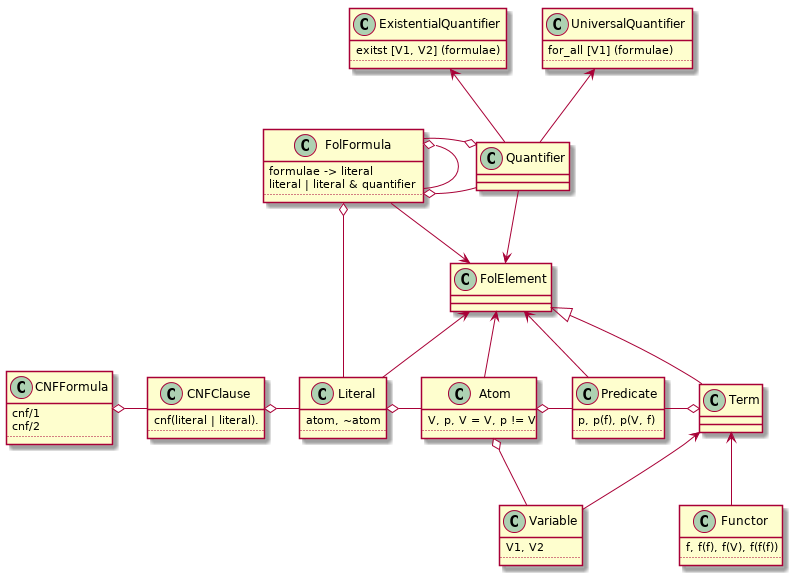
\includegraphics[width=\textwidth]{logic-formula-generator/fol/fol_elements.png}
\end{centering}

\section{CNF Generator parameters}

User defines generator in 3 steps.

\subsection{Allowed FOL elements}

In this step user defines set of allowed \gls{FOL} elements:
\begin{itemize}
	\item set of allowed functor arities $a_f = \{0, 1, 2,\dots\}$
	\item maximum recursion depth $n$ for functors
	\item set of allowed predicate arities $a_p = \{0, 1, 2,\dots\}$
	\item set of atom allowed connectives, that is no connective or/and any subset of $AllowedConnectives = \{=, !=\}$
	\item if negated literals are allowed
	\item set of allowed clause lengths $AllowedClausesLen = \{1,2,\dots\}$
	\item set of allowed number of clauses in formula $AllowedFormulaLen = \{1,2,\dots\}$
\end{itemize}

\subsection{Number of each element}
In this step iser defines what properties formula should have:
\begin{itemize}
	\item formula contains from $c_{min}$ to $c_{max}$ clauses, but the best solution is considered middle of this range
	\item formula contains from $l_{min}$ to $l_{max}$ literals, but the best solution is considered middle of this range
	\item TODO more params
\end{itemize}

\subsection{Names}
In this step user defines:
\begin{itemize}
	\item set of variable names $\{'v1','v2',\dots\}$
	\item set of functor names $\{'f1','f2',\dots\}$
	\item set of predicate names $\{'p1','p2',\dots\}$
\end{itemize}


\section{Basic algorithm}

The basic algorithm is greedy:
\begin{enumerate}
	\item Generate all possible formulas, based on user given values
	\item Pick first one that matches requirements
\end{enumerate}

Although presented algorithm is greedy, it can be optimized by solving equasions, that define user requirements.

\section{Optimizations}

CNF formula $F_{cnf}$ consists of clauses $c1, c2, \dots$. The order of clauses in not important.

\begin{align*}
	&F_{cnf}(x) = \{c1, c2, \dots\, cx\} \\
	\text{where }
		&x \text{ -- number of clauses in formula}
\end{align*}

If we group clauses by their length:
\begin{align*}
	&F_{cnf}(x) = \bigcup_{i=1}^c c_i \\
	\text{where }
		&c_i \text{ -- set of clauses with length i}
\end{align*}

Number of literals in formula can be represented as:
\begin{align*}
	l(x) &= x_1|c_1| + x_2|c_2| + \dots + x_x|c_x| = \sum_{i=1}^{x} x_i |c_i| \\
	x &= x_1 + x_2 + \dots + x_n \\
	c_i &\in AllowedClausesLen, \forall_{i,j} c^i \neq c^j  \\
	\text{where }
		&x \text{ -- number of clauses in formula} \\
		&l(x) \text{ -- number of literals in formula} \\
		&|c_i| \text{ -- number of clauses with length i} \\
\end{align*}

By solving above equation we can reduce greedyness of algorithm. By using integer programming we can solve following equation within user defined thresholds and return random formula.

\begin{align*}
	l(x) &= \sum_{i=1}^{x} x_i |c_i| \\
	x &= \sum_i^x x_i \\
	l_{min} &< l(x) < l_{max} \\
	c_{min} &< x < c_{max} \\
	\text{where }
		&x \text{ -- number of clauses in formula} \\
		&l(x) \text{ -- number of literals in formula} \\
		&|c_i| \text{ -- number of clauses with length i} \\
\end{align*}

\section{Complexity}

\subsection{Number of functors}

Functor can contain variable or another functor.

How many types (ignore functor and variable names) of functors $f$ can be produced, knowing that
\begin{itemize}
	\item $n$ is recursion depth,
	\item $a$ is arity,
	\item subfunctors have arity less or equal to $a$?
\end{itemize}


\begin{align*}
	&f(n, a) =
	\begin{cases}
		a, \text{for } n = 0, \\
		a \sum_{i=n}^{i=1} \sum_{j=a}^{j=0} f(n-i,a-j) \\
	\end{cases} \\
\end{align*}

\subsection{Number of predicates}

Predicates can contain functors or variables.

How many types (ignoring predicate, functor and variable name) of predicates $P$ can be produced, knowing that:
\begin{itemize}
	\item functor arity $a_f$ is in range $[a_{f1}, a_{f2}]$,
	\item functor recursion depth $n$ is less or equal to $n_{max}$,
	\item $a_p$ is predicate arity?
\end{itemize}

\begin{align*}
	f_t(n_{max}, a_{fmin}, a_{fmax}) &= \sum_{i=0}^{n_{max}} \sum_{j=a_{f1}}^{a_{f2}} f(i, j), \\
	P(a_p) &=
	\begin{cases}
		1, \text{for } a_p = 0 \\
		(f_t(n_{max}, a_{fmin}, a_{fmax}) + 1)^{a_p}, \\
	\end{cases} \\
	\text{where} \\
	f_t(n_{max}, a_{fmin}, a_{fmax}) & \text{ -- total number of functors} \\
\end{align*}

\subsection{Number of atoms}

Atom can contain variabe or predicate. Atom connects items with binary mathematical connective: $=$ or $!=$.

How many types of atoms $A$ can be produced, knowing that:
\begin{itemize}
	\item predicate arity $a_p$ is given as set of $\{1,2,\dots\}$?
\end{itemize}

\begin{align*}
	A(a_p) &=
	\text{where} \\
	& \text{ -- total number of functors} \\
\end{align*}

\subsection{Number of literals}

\subsection{Number of clauses}

Clause $C$ can contain only literals. The order of literals is not important.

\begin{align*}
	&C = \{l1, 12, \dots\}
\end{align*}

How many different clauses can be produced, knowing that:
\begin{itemize}
	\item clause length is $x$
	\item given set of literals $L = \{l1, l2, \dots\}$, $\forall_{i,j \in L} i \neq j$
\end{itemize}

\begin{align*}
	&C(x) = \binom{|L|}{x}, \\
	\text{where }
	&|L| \text{ -- number of elements in L} \\
\end{align*}

\subsection{Number of cnf formulas}

How many different cnf formulas can be produced, knowing that:
\begin{itemize}
	\item formula contains $x$ clauses
	\item given set of clauses $C = \{c1, c2, \dots\}$, $\forall_{i,j \in L} i \neq j$
\end{itemize}

\begin{align*}
	&F_{cnf}(x) = \binom{|C|}{x}, \\
	\text{where }
	&|C| \text{ -- number of elements in C} \\
\end{align*}



% itd.
% \appendix
% \include{dodatekA}
% \include{dodatekB}
% itd.

\printglossary

\printbibliography

\end{document}
